\chapter{Windows Desktop-Anwendung zur Steuerung des Treibers}
\label{chap:WindowsDesktop-AnwendungzurSteuerungdesTreibers}

%Setzen der Schriftgröße für die Code-Beispiele von Manuel
\lstset{basicstyle=\normalsize}

Um unseren Treiber einfach bedienen zu können, haben wir eine grafische Benutzeroberfläche, kurz GUI, entwickelt. Durch ein simples und intuitives Design ermöglicht unsere Desktop-Anwendung das Verbinden mit einem Server, das Einsehen der aktuellen Netzgeschwindigkeit, sowie das Tätigen von Einstellungen mit nur wenigen Mausklicks. 
\\ \ \\
Anhand der in Kapitel 3.1.3 beschriebenen Vor-und Nachteile haben wir uns dazu entschieden, unsere grafische Benutzeroberfläche mit Windows Forms zu programmieren.
Das GUI-Framework WPF bietet zwar eine größere Freiheit im Bezug auf das Designen, aber dadurch kann das Implementieren auch schnell unnötig kompliziert und aufwändig werden. Das Problem, das man bei der Auswahl der Elemente auf die Standard-Windows-Benutzerelemente beschränkt ist, kann mit einigen Tricks umgangen werden, sodass auch in WinForms die Bedienelemente komplett nach seinen eigenen Wünschen umgebaut und redesignet werden können.

\section{Design und Funktionalität der Desktop-Anwendung}

\subsection{Design und Funktionalität der Hauptseite}

Nach dem Öffnen der Desktop-Anwendung soll es für den Benutzer möglich sein, eine Verbindung mit dem aus der Liste ausgewählten Server herzustellen beziehungsweise auch wieder die Verbindung zu trennen. Somit ist klar, dass wir für diese Funktionalität drei verschiedene Zustände benötigen:
\\
\begin{itemize}
 \item \textbf{Not Connected} (Nicht verbunden)
 \item \textbf{Connecting} (Verbinden)
 \item \textbf{Connected} (Verbunden)
\end{itemize}
\bigskip

\subsubsection{Grafikdesign}

Um den aktuellen Verbindungszustand zu visualisieren, haben wir mithilfe von GIMP drei unterschiedliche Symbole erstellt. Jeder der drei Zustände soll ein jeweils eigenes Erscheinungsbild in Form von verschiedenen Farben, Animationen, sowie Funktionalitäten haben. 
\\ \ \\
Das Herstellen der Verbindung mit einem Server wird mithilfe einer Ladeanimation verbildlicht. Diese Animation wurde mit dem in GIMP integrierten GIF-Animator kreiert. Hierbei muss für jeden Frame des GIFs eine eigene Ebene erstellt werden. Wichtig ist, dass jede Ebene einen Name sowie eine positive Zahl in der Größeneinheit Millisekunden haben muss. Somit weis GIMP wie lang ein bestimmter Frame angezeigt werden soll. Beim exportieren muss noch angegeben werden, dass es sich bei den erstellten Einzelframes um eine Animation handelt. Weiters können noch Einstellungen über Pausen, Übergänge und Endlosschleifen getätigt werden.\footnote[1]{\cite[Vgl.][]{GIF}}
\\ \ \\
In Abbildung 7.1 sieht man die Symbole der drei Zustände. Von links nach rechts symbolisieren sie Not Connected, Connecting und Connected.
\\
\begin{figure}[H]
    \centering
    
\includegraphics[width=0.6\textwidth]{Connection-Symbols.png}
    \caption{Symbole der Verbindungszustände} 
\end{figure}
\noindent
Neben dem Verbindungszustand wird auch die aktuelle Internetgeschwindigkeit in Form von verschiedenen Symbolen, welche in Figma erstellt wurden, angezeigt.
\\ \ \\
In Abbildung 7.2 sind die Symbole der Internetgeschwindigkeit von keiner Verbindung bis hin zur einer schnellen Internetgeschwindigkeit dargestellt.
\\
\begin{figure}[H]
    \centering
    
\includegraphics[width=0.4\textwidth]{Speed-Symbols.png}
    \caption{Verschiedene Symbole der Internetgeschwindigkeit} 
\end{figure}

\pagebreak

\subsubsection{Design des Zustandes Not Connected}

Der Startzustand, welcher direkt nach dem Öffnen der Desktop-Anwendung angezeigt wird ist der Not Connected-Zustand. In diesem Zustand wird der Hintergrund mit der Farbe Rot angezeigt. Das Textfeld in der Mitte der Anwendung zeigt hierbei immer den aktuellen Zustand, in diesem Fall Not Connected, an. Weiters lassen das ausgegraute Verbindungssymbol in der Mitte, sowie das durchgestrichene Geschwindigkeitssymbol am rechten oberen Rand darauf schließen, dass man aktuell mit keinem Server verbunden ist.
Der im unteren Teil der Desktop-Anwendung befindliche Connect-Button zeigt dem Benutzer mit dem Text Select Server, dass ein Server zum Verbinden ausgewählt werden muss.
\\ \ \\
Mit einem Klick auf den Pfeil, welcher sich auf der rechten Seite des Connect-Buttons befindet, öffnet sich eine DropUp-Liste mit allen zuvor im Menü hinzugefügten Servern. Nachdem man den gewünschten Server ausgewählt hat ändert sich die Farbe des Button auf intensiveres Grün und der Text auf Connect to \textit{Servername}. Hiermit wird dem Benutzer signalisiert, dass nun durch einen Mausklick auf die Mitte des Buttons der Verbindungsaufbau mit dem gewählten Server gestartet werden kann.
\\
\begin{figure}[H]
    \centering
    \setlength{\fboxsep}{1pt}
	\setlength{\fboxrule}{1pt}
	\fbox{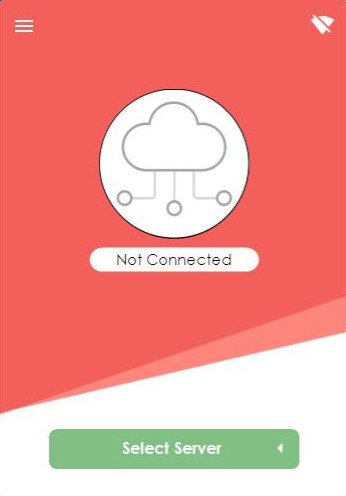
\includegraphics[width=0.4\textwidth]{NotConnected.jpg}}
    \caption{Design der Desktop-Anwendung im Zustand Not Connected} 
\end{figure}

\pagebreak

\subsubsection{Design des Zustandes Connecting}

Startet der Benutzer den Verbindungsaufbau, wechselt die Desktop-Anwendung in den Zustand Connecting. Hier wird der Hintergrund in der Farbe Blau angezeigt. Weiters ändert sich die Farbe des Buttons zu Grau und der Pfeil, welcher die Serverauswahl öffnet, verschwindet. Somit kann in der Zeit des Verbindens kein neuer Server ausgewählt werden. Auch kann nicht auf das Menü-Icon, welches die Einstellungen öffnet, gedrückt werden. Das Textfeld in der Mitte der Anwendung zeigt nun Connecting an und die animierte Ladeanimation deutet darauf hin, dass sich der Treiber mit dem ausgewählten Server verbindet.
\\
\begin{figure}[H]
    \centering
    \setlength{\fboxsep}{1pt}
	\setlength{\fboxrule}{1pt}
	\fbox{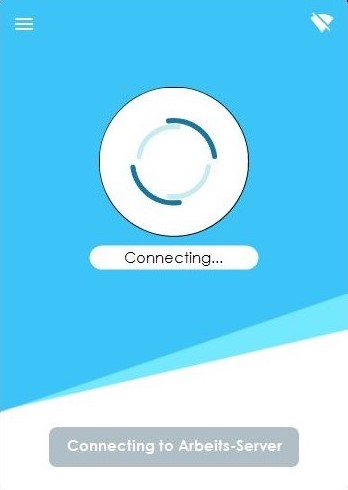
\includegraphics[width=0.4\textwidth]{Connecting.jpg}}
    \caption{Design der Desktop-Anwendung im Zustand Connecting} 
\end{figure}

\subsubsection{Design des Zustandes Connected}

Nach einem erfolgreichen Verbindungsaufbau wechselt die Desktop-Anwendung in den dritten Zustand Connected. In diesem Zustand wird der Hintergrund in der Farbe Grün angezeigt. Das Textfeld in der Mitte der Anwendung sagt nun “Connected to Servername”. Weiters lässt das darüberliegende Verbindungssymbol darauf schließen, dass man mit dem Server verbunden ist. Der Connect-Button hat sich auf die Farbe Rot und der Text auf Disconnect geändert. Das im rechten oberen Eck der Desktop-Anwendung befindliche Internetgeschwindigkeitssymbol hat neben der visuellen Darstellung nun auch eine weitere Funktion. Wenn man mit der Maus über das Symbol fährt erscheint links daneben eine Anzeige, welches dem Benutzer Auskunft über die aktuelle Internetgeschwindigkeit im Format Megabit pro Sekunde sowie den aktuellen Ping im Format Millisekunden gibt.
\\
\begin{figure}[H]
    \centering
    \setlength{\fboxsep}{1pt}
	\setlength{\fboxrule}{1pt}
	\fbox{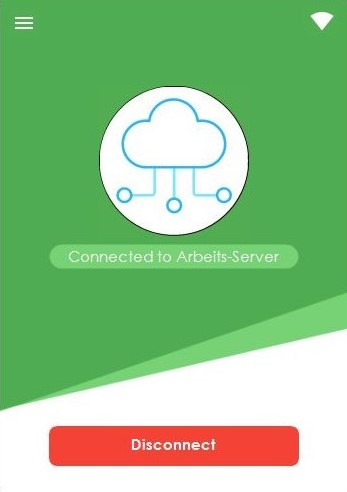
\includegraphics[width=0.4\textwidth]{Connected.jpg}}
    \caption{Design der Desktop-Anwendung im Zustand Conneted} 
\end{figure}

\subsubsection{Design des Fensters}

Viele Komponenten der Desktop-Anwendung wie Buttons und Textfelder haben ein modernes Design mit abgerundeten Ecken. Um eine einheitliche Designsprache zu gewährleisten soll auch das Fenster runde Ecken bekommen. Hierfür muss die Dynamic Link Library Gdi32\footnote[1]{\cite[Vgl.][]{GDI}} von Windows importiert werden. Diese beinhaltet die Methode \mbox{CreateRoundRectRgn()}, mit welchem ein neues Fenster mit angegebener Ellipsengröße für die Ecken erstellt werden kann.

\begin{program}[H]
\begin{CSharpCode}
Region = Region.FromHrgn(CreateRoundRectRgn(0, 0, Width, Height, 10, 10));
\end{CSharpCode}
\caption{Erstellen eines neuen Fensters mit abgerundeten Ecken}
\end{program}

\subsection{Design und Funktionalität des Connect-Buttons}

Der Connect-Button ist einer der wichtigsten Elemente der Desktop-Anwendung. Mithilfe diesem ist es möglich einen Server auszuwählen und sich mit diesem zu verbinden. Nach einem erfolgreichen Verbindungsaufbau kann man mit dem selben Button die Verbindung zum Server wieder trennen. Zusätzlich zur beschriebenen Funktionalität soll das Bedienelement über ein modernes Design mit abgerundeten Ecken verfügen.
\\ \ \\
Möchte man nun einen Button mit genau diesen Anforderungen in die Realität umsetzen, stößt man in WinForms mit den Standard-Windows-Bedienelementen auf drei wesentliche Probleme.
\\
\begin{enumerate}
 \item Der Standard-Button von WinForms ist viereckig und es gibt keine Möglichkeit dies zu ändern.
 \item Der Button soll über ein DropUp-Menü verfügen, welches eine Liste von Servern beinhaltet. Weiters soll man durch einen Mausklick auf diesen einen der Server auswählen können um sich damit zu verbinden. WinForms bietet zwar für solche Fälle eine sogenannte ComboBox an, doch diese hat erstens nur ein DropDown-Menü und zweitens stößt man bei der Benutzung dieser Komponente auf ein weiteres, nun folgendes Problem.
 \item Der Button soll zweigeteilt sein. Das bedeutet dass durch das Klicken auf das Bedienelement einerseits das Verbinden mit einem Server, andererseit aber auch das Öffnen des DropUp-Menüs möglich sein muss. Somit muss je nach Position des Mauszeigers beim Klick auf den Button eine andere Funktionalität verfügbar sein was mit dem Standard-Button ebenfalls nicht umsetzbar ist.
\end{enumerate}
\ \\
Die von uns verwendete Dynamic Link Library MetroSuite bietet zwar einen eigenen sogenannten MetroButton bei welchem man per Einstellung die Kanten abrunden kann, doch die 2 anderen Probleme können auch mit der Benutzung der DLL nicht gelöst werden. Daher können wir die Standard-Windows-Bedienelemente nicht benutzen und müssen einen eigenen Button programmieren.
\\ \ \\
In Abbildung 7.6 sind das gewünschte Design und die Funktionalität des Connect-Buttons dargestellt.
\begin{figure}[H]
    \centering
    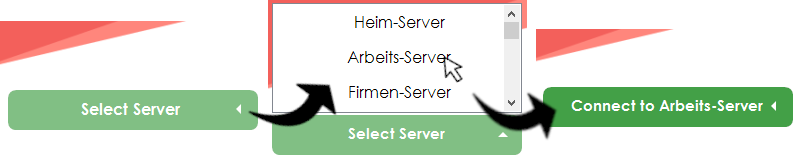
\includegraphics[width=1\textwidth]{connectButton.png}
    \caption{Design und Funktionalität des Connect-Buttons} 
\end{figure}

\subsubsection{Inhalt der Klasse Connect-Button}

Um einen eigenen Button mit unseren Wünschen zu kreieren, haben wir eine eigene Klasse namens ConnectButton, welche von der Standard-Button-Klasse abgeleitet ist, geschrieben. Die Button-Klasse ist Teil des System.Windows.Form-Namespaces, welcher alle User-Interface-Komponenten von Windows beinhaltet. Somit benutzen wir die schon vorhandenen Funktionalitäten eines Windows-Buttons und ergänzen diese mit eigenen zusätzlichen Funktionen und einem neuen Design.
\\ \ \\
Zum Designen des neuen Buttons benutzen wir die Klasse GraphicsPath, welche Teil vom System.Drawing.Drawing2D-Namespace ist. Mithilfe dieser Klasse ist es möglich Formen und Figuren mit der integrierten Grafik-Engine zu erstellen. Hierfür stellt die Klasse eine Reihe an Methoden zur Verfügung, mit welchen man neue Formen zu seiner Figur hinzufügen kann. In unseren Fall wurde die beiden Methoden AddLine() und AddArc() verwendet. Mithilfe dieser konnte die Form eines Buttons mit vier Linien und vier runden Ecken nachgebildet werden.

\begin{program}[H]
\begin{CSharpCode}
GraphicsPath graphPath = new GraphicsPath();
graphPath.AddLine(x1, y1, x2, y2);
\end{CSharpCode}
\caption{Hinzufügen einer Linie zu einer Figur}
\end{program}
\noindent 
Damit die erstellte Figure auch gezeichnet wird, muss noch die OnPaint-Methode der abgeleiteten Klasse Button überschrieben werden. In dieser Methode würde normalerweise der Standard-Windows-Button gezeichnet werden. Da hier aber jetzt unsere eigene Figure gezeichnet werden soll löschen wir das bestehende Design und zeichnen mit der Methode FillPath() die neue Figur.

\begin{program}[H]
\begin{CSharpCode}
protected override void OnPaint(PaintEventArgs paintEvent)
{
    paintEvent.Graphics.FillPath(brush, graphPath);
}
\end{CSharpCode}
\caption{Zeichnen einer Figur}
\end{program}
\noindent 
Wenn man nun den Connect-Button erstellt wird man bemerken, dass dieser vor allem in den Ecken nicht schön rund sondern eher verpixelt von der Grafik-Engine gezeichnet wurde. Um diesem Problem entgegenzuwirken müssen in der OnPaint()-Methode noch einige Einstellungen über die Renderqualität getätigt werden.

\begin{program}[H]
\begin{CSharpCode}
paintEvent.Graphics.InterpolationMode = InterpolationMode.HighQualityBilinear;
paintEvent.Graphics.CompositingQuality = CompositingQuality.HighQuality;
paintEvent.Graphics.PixelOffsetMode = PixelOffsetMode.HighQuality;
paintEvent.Graphics.SmoothingMode = SmoothingMode.AntiAlias;
\end{CSharpCode}
\caption{Beispiel-Code zum Verbessern der Renderqualität}
\end{program}
\noindent 
Mithilfe dieser vier Methoden werden alle wichtigen, für die Zeichen- und Renderqualität verantwortlichen Parameter auf die maximale Qualität gestellt um die bestmögliche Grafik zu erzielen. 
\\ \ \\
Neben einem Text soll auf der rechten Seite des Connect-Buttons auch ein Pfeil angezeigt werden, welcher dem Benutzer zeigt, dass man mit einem Mausklick auf diesen die Drop-Up-Liste öffnen beziehungsweise schließen kann. Dieser Pfeil soll je nachdem ob die Liste gerade geöffnet oder geschlossen ist, nach oben oder nach links zeigen. Hierfür wurden zwei verschiedene Pfeile für die beiden Richtungen in Figma kreiert. Die beiden Grafiken werden mithilfe der Klasse Icon eingelesen und können dann mit der Methode DrawIcon() an einer bestimmten Stelle im Button gezeichnet werden. Wichtig hierbei ist, dass die eingebundenen Icons vom Typ .ico sein müssen! 

\begin{program}[H]
\begin{CSharpCode}
Icon arrow = new Icon("arrow.ico");
paintEvent.Graphics.DrawIcon(arrow , x, y);
\end{CSharpCode}
\caption{Zeichnen eines Icons}
\end{program}
\noindent 
Da der Connect-Button durch das Klicken auf zwei verschiedene Stellen zwei verschiedene Funktionalitäten haben soll muss hier mit der Position des Mauszeigers beim Klick gearbeitet werden. Zuerst wird ein MouseUp-Event definiert, welches beim wieder Loslassen nach dem Drücken der linken Maustaste aktiviert wird. Nun kann mit MousePosition.X die X-Koordinate der aktuellen Position des Mauszeigers abgerufen werden. Mithilfe dieser Koordinate kann man überprüfen ob der Benutzer die Drop-Up-List aufrufen oder den Verbindungsaufbau starten möchte. Falls noch kein Server ausgewählt worden ist, ist der Mausklick zum Verbinden wirkungslos.

\subsubsection{Design und Funktionalität der Drop-Up-Liste}

Die Drop-Up-Liste soll die Möglichkeit bieten einen Server auszuwählen, um sich mit diesem zu verbinden. Hierfür verwenden wir die ListBox von WinForms. Diese Komponente ermöglicht standardmäßig das Hinzufügen von Einträgen, das Auswählen dieser, sowie das Nutzen einer Scrollbar. Zusätzlich dazu wurde auch dieses UI-Element an unserer Wünsche angepasst und um einige Funktionalitäten erweitert. Das Ziel ist, genauso wie beim Connect-Button, das Design zu verbessern. Die Änderungen umfassen das Anpassen der Schriftart/-größe und der Position, sowie das Verhalten beim Auswählen eines Servers durch einen Mausklick auf diesen.
\\ \ \\
Um die gewünschten Änderungen umzusetzen muss nicht wie beim Connect-Button eine eigene Klasse erstellt und die OnPaint()-Methode überschrieben werden. Hierfür gibt es das ListBox-Event DrawItem. Mithilfe von Events und Delegates ist es also möglich eine eigene Methode zu schreiben, mit welcher man die Elemente der ListBox selbst zeichnen kann. Wichtig zu erwähnen ist, dass wenn man diese Methode verwenden möchte, vorher noch die Option DrawMode der ListBox auf OwnerDrawFixed gestellt werden muss!
\\ \ \\
Nun haben wir die Möglichkeit, das Verhalten beim Auswählen eines Listenelementes zu definieren. Hierfür wird mit einem If-Anweisung überprüft ob das Listenelement ausgewählt wurde. Falls das der Fall ist, wird die Schriftart auf Fett geändert und die Schriftfarbe auf Grün.

\begin{program}[H]
\begin{CSharpCode}
if (drawEvent.State == DrawItemState.Selected)
{
    drawEvent = new DrawItemEventArgs(/*Parameter*/);
}
\end{CSharpCode}
\caption{Ändern der Eigenschaften eines ausgewählten Listenelements}
\end{program}
\noindent
Nach dem Definieren aller weiteren Parameter, wie Standard-Schriftart, -farbe und -größe muss das Listenelement noch gezeichnet werden. Hierfür kommt die Methode DrawString() zum Einsatz. Da hier auch Informationen über die Position angegeben werden müssen, kann so auch gleich definiert werden, dass das Element mittig in der ListBox zentriert gezeichnet werden soll.

\begin{program}[H]
\begin{CSharpCode}
drawEvent.Graphics.DrawString(text, font, brush, x, y);
\end{CSharpCode}
\caption{Zeichnen eines Listenelementes}
\end{program}
\noindent
Zum Einstellen des Abstandes zwischen den Listenelementen gibt es die ListBox-Eigenschaft ItemHeight. Mithilfe dieser kann der gewünschte Wert definiert werden. Hierfür muss aber die Option DrawMode der ListBox auf OwnerDrawVariable gestellt werden.

\subsection{Design und Funktionalität des Menüs}
Mit einem Mausklick auf das Icon in der linken oberen Ecke der Desktop-Anwendung gelangt man in das Menü. Hier können wichtige Einstellungen getätigt werden. Das Menü ist in die drei Menüpunkte Mode, Server und Network Devices unterteilt. Jeder der Menüpunkte wird durch ein eigenes, zur Einstellungsmöglichkeit passendes, Icon repräsentiert. Diese wurden in Figma erstellt. Mit einem Klick auf den jeweiligen Unterpunkt kommt man zu deren spezifischen Einstellungen. Um das Menü wieder zu verlassen, muss man auf den Schließen-Button, welcher sich oben links befindet klicken.
\\
\begin{figure}[H]
    \centering
    \setlength{\fboxsep}{1pt}
	\setlength{\fboxrule}{1pt}
	\fbox{\includegraphics[width=0.4\textwidth]{Menü.jpg}}
    \caption{Design des Menüs mit den drei Menüpunkten} 
\end{figure}

\pagebreak
\subsubsection{Design des Menüpunktes Mode}

Bei den Modus-Einstellungen, kann man definieren in welchem Modus der Treiber laufen soll. Man soll zwischen dem Perfomance-basierenden und Kostenbasierenden Modus auswählen können. Da wir uns im Rahmen der Diplomarbeit ausschließlich auf den ersten der beiden Modis konzentrieren dient der Menüpunkt Mode aktuell nur als Beschreibung des Kosten-basierenden Modus. Der ausgegraute Button mit dem Text “Selected” unterhalb der Kurzbeschreibung zeigt dem Benutzer, dass akutell dieser Modus ausgewählt ist. Mit einem Klick Mausklick auf den Pfeil links oben kommt man wieder in die Einstellungsübersicht zurück.
\\
\begin{figure}[H]
    \centering
    \setlength{\fboxsep}{1pt}
	\setlength{\fboxrule}{1pt}
	\fbox{\includegraphics[width=0.4\textwidth]{MenüMode.jpg}}
    \caption{Design des Menüpunktes Mode} 
\end{figure}

\subsubsection{Design des Menüpunktes Server}

Bei den Server-Einstellungen hat der Benutzer die Möglichkeit, Server zu verwalten.
Im oberen Bereich mit der Aufschrift “Add Server” kann man einen neuen Server hinzuzufügen. Hier muss der Name, welcher frei wählbar ist, die IP-Adresse und der Post des Servers eingetragen werden. Mit einem Klick auf “Add” wird der Server in die darunterliegende Liste hinzugefügt. Im unteren Bereich namens “Server List” werden alle gespeicherten Server angezeigt. Mit einem Mausklick auf einen Server wird die Schriftart Fett und die Schriftfarbe Blau angezeigt. Somit wurde der Server als Default-Server festgelegt. Mit dem Löschen-Button, welcher sich unterhalb der Liste befindet, kann ein ausgewählter Server wieder von der Liste entfernt werden.
\\
\begin{figure}[H]
    \centering
    \setlength{\fboxsep}{1pt}
	\setlength{\fboxrule}{1pt}
	\fbox{\includegraphics[width=0.4\textwidth]{MenüServer.jpg}}
    \caption{Design des Menüpunktes Server} 
\end{figure}
\noindent
WinForms bietet keine Möglichkeit, das Verhalten bei der Auswahl eines Listenelementes zu ändern. Daher kamen genauso wie bei der Drop-Up-Liste des ConnectButtons Event, Delegates und die Methode DrawItem() zum Einsatz um die Listenelement manuell zu zeichnen. Nur so konnte das Ändern der Schrifteigenschaften möglich gemacht werden.

\subsubsection{Speichern der Serverliste}
Da zur Serverliste hinzugefügte Server auch nach dem Schließen und einem erneuten Öffnen der Desktop-Anwendung noch zur Verfügung stehen sollen, müssen wichtige Einstellungen wie die Serverliste gespeichert werden. Hierfür benutzen wird den System.Text.Json-Namespace welcher es ermöglicht, Objekte ins JSON-Format zu serialisieren und vom JSON-Format wieder in Objekte zu deserialisieren.
\\ \ \\
Zur Speicherung relevante ist eine Liste mit allen Servern, welche wiederum aus den drei Attributen Name, IP-Adresse und Port bestehen. Um diese Daten einfach zu speichern und später wieder auslesen zu können haben wir eine Klasse namens ServerObject erstellt, welche die drei Attribute beinhaltet. Eine zweite Klasse ServerSettings speichert diese Server-Objekte in einer Liste.

\begin{program}[H]
\begin{CSharpCode}
public class ServerObject
{
    public string name { get; set; }
    public string ip { get; set; }
    public int port { get; set; }
}
\end{CSharpCode}
\caption{Aufbau der Klasse ServerObject}
\end{program}
\noindent
Wird nun ein neuer Server in der Desktop-Anwendung hinzugefügt, wird ein neues Server-Objekt erstellt und in die Serverliste hinzugefügt. Sollte ein bestehender Server gelöscht werden, wird das Server-Objekt wieder aus der Liste entfernt.
\\ \ \\
Schließt der Benutzer nun die Desktop-Anwendung werden mögliche Änderungen in der Serverliste gespeichert werden. Hierfür kommt der im System.Text.Json-Namespace enthaltene JsonSerializer zum Einsatz. Dieser serialisiert ein ServerSettings-Objekt, welches die Liste mit allen Servern-Objekten beinhaltet, zu einem JSON-Text. Dieser wird dann in eine Datei names serverSettings.json im selben Verzeichnis wo auch die .exe-Datei liegt gespeichert.

\begin{program}[H]
\begin{CSharpCode}
public class ServerObject
string settings = JsonSerializer.Serialize(serverSettings);
\end{CSharpCode}
\caption{Serialisieren des serverSettings-Objektes}
\end{program}
\noindent
Startet der Benutzer die Desktop-Anwendung, werden alle gespeicherten Einstellungen wieder geladen. Hierfür wird der gespeicherte JSON-Text aus der Datei ausgelesen und mit dem JsonSerializer deserialisiert.

\begin{program}[H]
\begin{CSharpCode}
serverSettings = JsonSerializer.Deserialize<ServerSettings>(settings);
\end{CSharpCode}
\caption{Deserialisieren des eingelesenen JSON-Textes}
\end{program}
\noindent
Nachdem das einlesen erfolgreich abgeschlossen wurde, werden die Serverliste im Menü sowie die Drop-Up-List vom Connect-Button mit den gespeicherten Einstellungen befüllt.

\subsubsection{Design des Menüpunktes Network Devices}

Bei den Netzwerkadapter-Einstellungen kann der Benutzer die Netzwerkadapter verwalten. Hierfür werden im Bereich mit der Aufschrift \grqq Network Devices List\grqq{} alle verfügbaren Netzwerkadapter aufgelistet. Durch einen Mausklick auf einen Listeneintrag wird die Schriftart Fett und die Schriftfarbe Blau. Somit wurde der Netzwerkadapter ausgewählt und wird nun vom Treiber verwendet. Mit einem erneuten Klick kann dieser auch wieder abgewählt werden. Für die Erweiterung des Kosten-basierenden Modus, würde noch die Angabe der Kosten pro Megabyte hinzukommen.
\\
\begin{figure}[H]
    \centering
    \setlength{\fboxsep}{1pt}
	\setlength{\fboxrule}{1pt}
	\fbox{\includegraphics[width=0.4\textwidth]{MenüNetworkDevices.jpg}}
    \caption{Design des Menüpunktes Network Devices} 
\end{figure}

\subsubsection{Einlesen der Netzwerkadapter}

Um die Netzwerkadapter auswählen zu können, müssen diese beim Start der Desktop-Anwendung eingelesen werden. Hierfür muss die Klasse Win32\_NetworkAdapterConfiguration instanziiert werden. Diese beinhaltet alle Attribute und Methoden der Netzwerkadapter. Das Attribut Description liefert uns den Namen des Netzwerkadapters, welchen wir in die Network-Devices-Liste speichern können. Mithilfe der Variable ipEnabled werden nur aktivierten Netzwerkadapter angezeigt.

\begin{program}[H]
\begin{CSharpCode}
if ((bool)managementObject["ipEnabled"])
{
    netDevices.Add(managementObject["Description"].ToString());
}
\end{CSharpCode}
\caption{Einlesen der Namen der aktiven Netzwerkadapter}
\end{program}
\noindent
Da die Namen der Netzwerkadapter oft zu breit für die Darstellung in der ListBox sind, muss gegebenenfalls eine horizontale Scrollbar angezeigt werden. Hierfür wird nach dem Einfügen der Adapter mithilfe der MeasureString()-Methode die Länge der Namen ermittelt.

%Setzen der Schriftgröße für die Code-Beispiele von Martin
\lstset{basicstyle=\footnotesize}

\pagebreak

\section{Desktop-Anwendung in der Notification Area}
Wir haben unsere Windows Desktop-Anwendung zum Steuern des Multi-Wan Bonding fähigen Treibers als Notification Area Programm entwickelt. Dabei war es uns sehr wichtig, dass der Benutzer einmal auf das Symbol klicken kann, damit wird ihm die wie im Kapitel 7.1 beschriebene Benutzeroberfläche angezeigt. Wenn er jetzt nochmals darauf oder woanders hin drückt, soll die Benutzeroberfläche verborgen werden
\\\\
Um eine Notification Area Anwendung zu implementieren, haben wir eine C\# Klasse entwickelt, diese Klasse ist von \textbf{ApplicationContext} abgeleitet. In dieser Klasse wird ein \textbf{NotifyIcon} angelegt. Dieses \textbf{NotifyIcon} benötigt ein Symbol, mit diesem wird dann die Anwendung in der Notfication Area abgelegt, einen Text der erscheint, sobald sich die Maus über dem Symbol befindet, in unserem Fall "NetShare". Weiters hat das Symbol einen Button zum Schließen der Anwendung, sobald das Symbol mit der rechten Maustaste angeklickt wurde. Wenn dieser Knopf gedrückt wird beendet sich die Windows Desktop-Anwendung und auch der Multi-Wan Bonding fähige Treiber.
\begin{figure}[H]
    \centering
    
\includegraphics[width=5cm, height=5cm, keepaspectratio]{NAIcon.png}
    \caption[NotificationArea]{Netshare Symbol in der Notification Area} 
\end{figure}
\noindent

\newpage
\subsection{Relative Positionierung der grafischen Oberfläche}
Die Grafische Oberfläche der Windows Desktop-Anwendung soll sich immer an der richtigen Stelle relativ zur Taskleiste positionieren. Mithilfe von \textbf{Screen.PrimaryScreen.Bounds} und \textbf{Screen.PrimaryScreen.WorkingArea} finden wir heraus wo sich die Taskleiste befindet. Mit diesem Wissen setzen wir dann die relative Positionierung der grafischen Oberfläche. \textbf{Screen.PrimaryScreen.Bounds} gibt einem die gesamte Größe des Bildschirms an, \textbf{Screen.PrimaryScreen.WorkingArea} gibt einem die Größe an in der z.B. auch Webbrowser geöffnet sind, also ohne der  Taskleiste. Im Codebeispiel sieht man wie dies funktioniert, wenn sich die Taskleiste am unteren Rand befindet.
\begin{program}[H]
\caption{Taskleiste unten}
\begin{CSharpCode}
if((Screen.PrimaryScreen.Bounds.Height - Screen.PrimaryScreen.WorkingArea.Height)>0)
{
    this.Location = new Point(Screen.PrimaryScreen.WorkingArea.X + 
      Screen.PrimaryScreen.WorkingArea.Width - Width - 10, 
      Screen.PrimaryScreen.WorkingArea.Y + Screen.PrimaryScreen.WorkingArea.Height 
      - Height);
}
\end{CSharpCode}
\end{program}
\noindent

\section{Kommunikation zwischen dem Multi-Wan Bonding fähigen Treiber und der Windows Desktop-Anwendung}
Die Windows-Desktop Anwendung muss für das Steuern des Multi-Wan Bonding fähigen Treibers mit diesem Kommunizieren. Wir haben uns als Interprozesskommunikationsart für Sockets entschieden, da wir dies für am einfachsten angesehen haben, weil man sich nicht um die Synchronisation kümmern muss. Der Multi-Wan Bonding fähige Treiber erstellt einen Server der auf "localhost" \ auf dem Port 5260 lauscht und wartet bis sich ein Client mit ihm verbindet. Die Windows Desktop-Anwendung erstellt für jeden Steuerungsbefehl an den Multi-Wan Bonding fähigen Treiber einen Client, der sich zum Server verbindet und dann ein JSON Objekt mit dem jeweiligen Befehl zum Server sendet. Sobald die Windows Desktop-Anwendung die erwartete Antwort bekommen hat, wird die Verbindung zum Multi-Wan Bonding fähigen Treiber geschlossen.

\newpage
\subsection{JSON Object}
\subsubsection{Anfrage (Request)}
Wenn die Windows Desktop-Anwendung eine Anfrage an den Multi-Wan Bonding fähigen Treiber sendet, hat das JSON Objekt folgende Struktur.
\begin{program}[H]
\caption{JSON Anfrage}
\begin{GenericCode}
    {
        "type" :  "",
        "on" :  "",
        "data" : {} 
    }
\end{GenericCode}
\end{program}
\noindent
Bei dem Schlüssel \textbf{type} wird vom Multi-Wan Bonding fähigen Treiber \textbf{Get} oder \textbf{Put} erwartet. Mit \textbf{Get} kann die Windows-Desktop Anwendung die derzeitige Konfiguration oder die Download und Upload Geschwindigkeiten des Multi-Wan Bonding fähigen Treibers anfordern. Mithilfe von \textbf{Put} werden Einstellungen hinzugefügt oder geändert. 
\\\\
Bei dem Schlüssel \textbf{on} gibt es die Werte \textbf{driver.state}, \textbf{deamon.state}, \textbf{connection.state}, \textbf{config} und \textbf{statistics}. Mit \textbf{driver.state} verbindet sich der Multi-Wan Bonding fähige Treiber mit dem Multi-Wan Bonding fähigen Server oder bricht die Verbindung ab. Mithilfe von \textbf{deamon.state} kann man den Multi-Wan Bonding fähigen Treiber beenden. Mit \textbf{connection.state} kann man die Verbindung zwischen dem Server und dem Client von der Server Seite aus beenden und mit \textbf{config} kann man die derzeitigen Konfigurationen anpassen oder anfordern. Mit dem Wert \textbf{statistics} erhält man die Download und Upload Geschwindingkeiten.
\\\\
Bei dem Schlüssel \textbf{data} wird der Wert \textbf{state} erwartet, falls bei dem Schlüssel on der Wert \textbf{driver.state}, \textbf{deamon.state} oder \textbf{connection.state} ist. Wenn der vorherige Schlüssel \textbf{config} ist, wird bei \textbf{data} entweder \textbf{logLevel}, \textbf{serverIp}, \textbf{adapterIp}, \textbf{adapterSubnetBits}, \textbf{names} oder nichts, falls man die gesamte Konfiguration erhalten will, dies ist aber nur möglich, wenn bei dem Schlüssel \textbf{type} der Wert \textbf{Get} ist. Wenn beim Schlüssel \textbf{on} \textbf{statistics} steht, ist wird in \textbf{data} ebenfalls nichts erwartet. 


\subsubsection{Antwort (Response)}
Wenn der Multi-Wan Bonding Server eine Antwort an die Windows-Desktop Anwendung sendet, ist das JSON Objekt folgendermaßen aufgebaut.
\begin{program}[H]
\caption{JSON Antwort}
\begin{GenericCode}
    {
        "type" :  "",
        "data" : {}
    }
\end{GenericCode}
\end{program}
\newpage
\noindent
Bei dem Schlüssel \textbf{type} gibt es zwei mögliche Werte entweder \textbf{Response} oder \textbf{Update}. Mit \textbf{Response} wird mitgeteilt das eine Anfrage fertig abgearbeitet ist. Mithilfe von \textbf{Update} wird ausgedrückt, dass der Multi-Wan Bonding fähige Treiber etwas geändert hat.
\\\\
Beim Schlüssel \textbf{data} steht, falls ein Fehler aufgetreten ist \textbf{error}, ansonsten \textbf{state}, der angeforderte Konfigurationswert, alle konfigurierten Werte mit dem jeweiligen Werten drinnen oder \textbf{down} mit einem Wert und \textbf{up} mit einem Wert.  


\subsection{Verbinden des Multi-Wan Bonding fähigen Treibers mit einem Multi-Wan Bonding fähigen Server}
Um mithilfe des Multi-Wan Bonding fähigen Treibers die Verbindung zum Multi-Wan Bonding fähigen Server herzustellen, wird eine Anfrage von der Windows-Desktop Anwendung gesendet. Diese Anfrage ist folgendermaßen aufgebaut:
\begin{program}[H]
\caption{JSON Anfrage verbinden}
\begin{GenericCode}
    {
        "type" :  "Put",
        "on" :  "driver.state",
        "data" : {"state" : "running"} 
    }    
\end{GenericCode}
\end{program}
\noindent
Daraufhin checkt der Multi-Wan Bonding fähige Treiber ob dieser schon mit dem Multi-Wan Bonding fähigen Server verbunden ist, falls dies der Fall ist, wird diese Antwort gesendet:
\begin{program}[H]
\caption{JSON Antwort verbinden running}
\begin{GenericCode}
    {
        "type" :  "Response",
        "data" : {"state" : "running"} 
    }    
\end{GenericCode}
\end{program}
\noindent
Falls der Multi-Wan Bonding fähige Treiber sich gerade mit dem Multi-Wan Bonding fähigen Server verbindet oder noch keine Verbindung aufgebaut ist, wird beim Schlüssel \textbf{state} der Wert \textbf{startup} eingetragen und als Antwort gesendet. Nachdem die Verbindung erfolgreich aufgebaut wurde, wird das JSON Objekt von vorher gesendet. Wenn die Verbindung nicht aufgebaut werden kann, bekommt man folgende Antwort:
\begin{program}[H]
\caption{JSON Antwort verbinden crashed}
\begin{GenericCode}
    {
        "type" :  "Response",
        "data" : {"state" : "crashed"} 
    }    
\end{GenericCode}
\end{program}
\newpage
\noindent
Nachdem man diese Antwort bekommen hat, versucht die Windows Desktop-Anwendung es noch zweimal, indem sie wieder die Anfrage an den Multi-Wan Bonding fähigen Treiber sendet. Falls bei den zwei weiteren Anfragen auch nur der Wert \textbf{crashed} bei dem Schlüssel \textbf{state} zurückkommt, wird dem Benutzer eine Fehlermeldung angezeigt, die Ihn dazu auffordert den Multi-Wan Bonding fähigen Treiber neu zu starten.


\subsection{Verbindung zu einem Multi-Wan Server trennen}
Um die Verbindung zwischen dem Multi-Wan Bonding fähigen Treiber und dem Multi-Wan Bonding fähigen Server zu trennen, wird eine Anfrage von der Windows Desktop-Anwendung gesendet. Diese Anfrage ist folgendermaßen aufgebaut:
\begin{program}[H]
\caption{JSON Anfrage Verbindung trennen}
\begin{GenericCode}
    {
        "type" :  "Put",
        "on" :  "driver.state",
        "data" : {"state" : "stopped"} 
    }     
\end{GenericCode}
\end{program}
\noindent
Der Multi-Wan Bonding fähige Treiber sendet als Antwort seinen derzeitigen Status, diese Antwort wird so gesendet:
\begin{program}[H]
\caption{JSON Antwort Verbindung trennen}
\begin{GenericCode}
    {
        "type" :  "Response",
        "data" : {"state" : ""} 
    }    
\end{GenericCode}
\end{program}
\noindent
Wobei bei dem Schlüssel \textbf{state} entweder der Wert \textbf{startup}, \textbf{running} oder \textbf{stopped} steht. Falls der Multi-Wan Bonding fähige Treiber als Status nicht \textbf{stopped} hat, bricht der Multi-Wan Bonding fähige Treiber die Verbindung zum Multi-Wan Bonding fähigen Server ab und sendet die Antwort an die Windows Desktop-Anwendung die als \textbf{state} \textbf{stopped} hat.


\subsection{Multi-Wan Bonding fähigen Treiber beenden}
Um den Multi-Wan Bonding fähigen Treiber zu beenden, wird eine Anfrage von der Windows Desktop-Anwendung gesendet. Diese Anfrage ist folgendermaßen aufgebaut:
\begin{program}[H]
\caption{JSON Anfrage Treiber beenden}
\begin{GenericCode}
    {
        "type" :  "Put",
        "on" :  "deamon.state",
        "data" : {"state" : "stopped"} 
    }     
\end{GenericCode}
\end{program}
\newpage
\noindent
Der Multi-Wan Bonding fähige Treiber sendet im Sekundentakt eine Antwort in dieser steht, was der Multi-Wan Bonding fähige Treiber gerade macht. Die Antwort wird mit diesem Aufbau gesendet:
\begin{program}[H]
\caption{JSON Antwort Treiber beenden}
\begin{GenericCode}
    {
        "type" :  "Update",
        "data" : {"state" : ""} 
    }    
\end{GenericCode}
\end{program}
\noindent
Bei dem Schlüssel \textbf{state} steht als Wert entweder \textbf{worker.startup}, \textbf{worker.running} oder \textbf{worker.stopped}. Solange sich der Multi-Wan Bonding fähige Treiber im Status \textbf{startup} befindet, passiert nichts außer, dass die Antwort mit \textbf{worker.startup} sekündlich gesendet wird. Sobald der Status \textbf{running} ist, wird die Antwort mit \textbf{worker.running} gesendet und die Anwendung bekommt den Befehl sich zu schließen. Wenn dies geschehen ist, wird die Antwort mit \textbf{worker.stopped} gesendet. Zusätzlich dazu wird noch eine Antwort gesendet die als \textbf{type} \textbf{Response} hat und bei \textbf{state} den Wert \textbf{stopped} hat.


\subsection{Konfiguration des Multi-Wan Bonding fähigen Treibers ändern}
Um die Einstellungen von dem Multi-Wan Bonding fähigen Treiber zu ändern, wird von der Windows Desktop-Anwendung eine Anfrage gesendet, die folgendermaßen aufgebaut ist:
\begin{program}[H]
\caption{JSON Anfrage Konfiguration ändern}
\begin{GenericCode}
    {
        "type" :  "Put",
        "on" :  "config",
        "data" : {} 
    }     
\end{GenericCode}
\end{program}
\noindent
Bei dem Schlüssel \textbf{data} wird das zu konfigurierende Schlüssel Wert Paar eingetragen. Der Multi-Wan Bonding fähige Treiber sendet als Antwort folgendes JSON-Objekt:
\begin{program}[H]
\caption{JSON Antwort Konfiguration ändern}
\begin{GenericCode}
    {
        "type" :  "Response",
        "data" : {} 
    }    
\end{GenericCode}
\end{program}
\noindent
In \textbf{data} steht das geänderte Schlüssel Wert Paar. Die einzige Änderung die der Multi-Wan Bonding fähige Treiber sofort übernimmt, ist eine Änderung beim \textbf{logLevel}. Jede andere Änderung wird erst verwendet nachdem die Verbindung zum Multi-Wan Bonding fähigen Server getrennt wurde und sich neu mit diesem Verbunden wurde.


\subsection{Konfiguration des Multi-Wan Bonding fähigen Treibers anfordern}
\subsubsection{Gesamte Konfiguration}
Um die gesamte Konfiguration des Multi-Wan Bonding fähigen Treibers zu bekommen, wird von der Windows Desktop-Anwendung eine Anfrage gesendet, die folgendermaßen aufgebaut ist:
\begin{program}[H]
\caption{JSON Anfrage Gesamte Konfiguration anfordern}
\begin{GenericCode}
    {
        "type" :  "Get",
        "on" :  "config",
        "data" : {} 
    }     
\end{GenericCode}
\end{program}
\noindent
Wenn diese Anfrage gesendet wird, antwortet der Multi-Wan Bonding fähige Treiber folgendermaßen:
\begin{program}[H]
\caption{JSON Antwort Gesamte Konfiguration anfordern}
\begin{GenericCode}
    {
        "type" :  "Response",
        "data" : {
                    "logLevel" : "",
                    "serverIp" : "",
                    "serverPort" : "",
                    "adapterIp" : "",
                    "adapterSubnetBits" : "",
                    "names" : []
        } 
    }    
\end{GenericCode}
\end{program}
\noindent
Bei jedem Schlüssel Wert Paar in \textbf{data} wird noch der eingestellte Wert eingetragen.


\subsubsection{Einzelne Einstellungen}
Um nur eine einzelne Konfiguration vom Multi-Wan Bonding fähigen Treiber zu bekommen, wird eine Anfrage von der Windows Desktop-Anwendung gesendet, die folgendermaßen aufgebaut ist:
\begin{program}[H]
\caption{JSON Anfrage einzelne Konfiguration anfordern}
\begin{GenericCode}
    {
        "type" :  "Get",
        "on" :  "config",
        "data" : {} 
    }     
\end{GenericCode}
\end{program}
\noindent
In dem Feld \textbf{data} steht ein Schlüssel Wert Paar als Schlüssel steht die gewünschte Option und als Wert eine Leere Zeichenkette. Der Multi-Wan Bonding fähige Treiber sendet eine Antwort die folgendermaßen Aufgebaut ist: 
\begin{program}[H]
\caption{JSON Antwort einzelne Konfiguration anfordern}
\begin{GenericCode}
    {
        "type" :  "Response",
        "data" : {} 
    }    
\end{GenericCode}
\end{program}
\noindent
In \textbf{data} steht das angeforderte Schlüssel Wert Paar.

\subsection{Upload und Download Geschwindigkeit anfordern}
Um in der Windows Desktop-Anwendung den Upload und den Download Speed anzeigen zu können, wird eine Anfrage an den Multi-Wan Bonding fähigen Treiber gesendet, diese Anfrage ist folgendermaßen aufgebaut:
\begin{program}[H]
\caption{JSON Anfrage Upload Download}
\begin{GenericCode}
    {
        "type" :  "Get",
        "on" :  "statistics",
        "data" : {} 
    }     
\end{GenericCode}
\end{program}
\noindent
Der Multi-Wan Bonding fähige Treiber sendet daraufhin jede Sekunde eine Antwort mit der Upload und Download Geschwindigkeit, diese werden kontinuierlich berechnet. Die Antwort ist folgendermaßen aufgebaut:
\begin{program}[H]
\caption{JSON Antwort Upload Download}
\begin{GenericCode}
    {
        "type" :  "Response",
        "data" : {
                    "down" : "",
                    "up" : ""
        } 
    }    
\end{GenericCode}
\end{program}
\noindent
Die Anfrage an den Mult-Wan Bonding fähigen Treiber wird automatisch gesendet, sobald dieser mit einem Multi-Wan Bonding fähigen Server verbunden ist. 

%Setzen der Schriftgröße für die Code-Beispiele für Manuel
\lstset{basicstyle=\normalsize}

\pagebreak

\section{Windows-Service zur Crash-Recovery des Treibers}

Ein Windows-Service, zu deutsch Windows-Systemdienst, ist ein Programm welches als Dienst im Hintergrund einer Windows-Sitzung läuft\footnote[1]{\cite[Vgl.][]{WindowsService}}. Somit eignet sich ein Windows-Service perfekt für unseren Treiber, welcher immer im Hintergrund laufen, aber den Benutzer nicht stören soll. Weiters soll dieser, bei einem möglichen Absturz, automatisch vom Service neu gestartet werden.

\subsection{Starten des Treibers}

Beim Starten unseres Treibers in Form einer .exe-Datei muss bedacht werden, dass seit der Windows Version Vista ein Windows-Service nicht mehr mit dem Desktop interagieren kann. Das bedeutet, dass der Systemdienst keine Programme mit grafischer Oberfläche starten kann. Da unser Treiber keine grafischen Elemente besitzt kann dieser mit der Angabe von zusätzlichen Parametern gestartet werden.
Mit dem Kofigurieren der Parameter CreateNoWindow und UseShellExecute weiß der Windows-Service, dass keine grafische Oberfläche sowie Shell vom Treiber benutzt wird.

\begin{program}[H]
\begin{CSharpCode}
ProcessStartInfo info = new ProcessStartInfo("netshare.exe");

info.UseShellExecute = false;
info.CreateNoWindow = true;
info.ErrorDialog = false;
info.WindowStyle = ProcessWindowStyle.Hidden;

Process process = Process.Start(info);
\end{CSharpCode}
\caption{Starten des Treibers mit Windows-Service}
\end{program}

\subsection{Crash-Recovery}

Damit sichergestellt werden kann, dass der Treiber immer verfügbar ist, muss im Windows-Service eine Crash-Recovery eingebaut werden. Diese überprüft ob das Programm noch läuft und startet gegebenenfalls den Treiber neu. Das laufende Programm kann mithilfe von \mbox{Process.GetProcessesByName("netshare.exe")} gefunden und somit überprüft werden.